\documentclass[xcolor=dvipsnames,10pt]{beamer}
% ********** Style prezentation **********

\usepackage{verbatim}
\usepackage{color}
\usepackage{multimedia}
\usepackage{xmpmulti}
\usepackage[absolute,overlay]{textpos} 
\usepackage{listings}
\usepackage{algorithm}
\usepackage{algorithmic}
\usepackage{amsmath}
\usepackage{pifont}
\usepackage{url}
\usepackage{pict2e}
\usepackage{flushend}
\usepackage{graphicx}
\usepackage{pgf}
\usepackage{url}
\usepackage{tikz}
\usetikzlibrary{calc}
\usetikzlibrary{shapes}
\usetikzlibrary{backgrounds}
\usepackage{pgfplots}
\usepackage{pgfplotstable}
\usepgfplotslibrary{fillbetween}


\newcommand{\ignore}[1]{}


\lstset{ %
  language=Java,              
  basicstyle=\footnotesize
}

\pgfdeclarelayer{foreground}
\pgfdeclarelayer{background}
\pgfsetlayers{background,main,foreground}

\mode<presentation>
{
	\usetheme{Warsaw}
}
\definecolor{scarlet}{RGB}{200,0,0}
\setbeamercolor{structure}{fg=scarlet}
\addtobeamertemplate{footline}{
\begin{columns}
  \hfill\includegraphics[height=.75cm]{unl_clear.pdf}\hspace{.5cm}
\end{columns}
\vspace{2mm}
}{\usebeamercolor[bg]{footline}\hfill\raisebox{1mm}[0mm]{\hspace{2mm}}}

\newcommand\x[1]{\ensuremath{\mathit{#1}}}
\newcommand\lrangle[1]{\ensuremath{\langle#1\rangle}}

\def\ON{\ding{52}}
\def\OF{\ding{55}}
\def~{\phantom{0}}

\setbeamertemplate{navigation symbols}{} %remove if navigation symbols are needed
\setbeamersize{text margin left=5mm, text margin right=5mm} % change margin as you wish

\author{Matthew B. Dwyer}

\title[Probabilistic Program Analysis]{Probabilistic Program Analysis}
\subtitle{GTTSE part 3}


\institute{
Department of Computer Science and Engineering\\
University of Nebraska - Lincoln\\
Lincoln, Nebraska USA\\
}

\date{August 2015}

\begin{document}

\begin{frame}
	\titlepage %displays the title page
\end{frame}


\pgfmathdeclarefunction{Gauss}{2}{%
  \pgfmathparse{1/(#2*sqrt(2*pi))*exp(-((\x-#1)^2)/(2*#2^2))}%
}

\pgfmathdeclarefunction{RightMirrorPiledGauss}{2}{%
 \pgfmathparse{x<0?0:2*Gauss(#1,#2)}%
}

\begin{frame}[fragile]
\frametitle{Adapting program analyses}
\vfill
As we have seen there are several well-developed program analysis frameworks
\vfill
Researchers have been exploring how to (minimally) adapt them to take probabilistic information into account
\begin{itemize}
\item reuse abstract domains and transformers in data flow analysis
\item reuse path generation and constraint optimization in sym. exe.
\end{itemize}
\vfill
\end{frame}

\begin{frame}[fragile]
\frametitle{Just enough probability}
\vfill
For simplicity we'll look at just the continuous case.
\begin{minipage}{0.45\textwidth}
\vfill
A probability \textit{density} function (pdf), $f$, 
defines the probability that a continuous random
variable takes on a specific value.
\mbox{~}\\
\mbox{~}\\
$Pr[a \le X \le b] = \int_{a}^{b} f(x) dx$ 
where $f$ is non-negative and Lebesgue-integrable
\mbox{~}\\
\mbox{~}\\
For $x$ drawn from $N(0,2)$:\\
\mbox{~~~}$Pr[-1 \le x \le 1]$ 
\end{minipage}%
\begin{minipage}{0.55\textwidth}
\mbox{~}\\
\mbox{~}\\
\mbox{~}\\
\mbox{~}\\
\mbox{~}\\
\begin{tikzpicture}[scale=0.75]
\begin{axis}[xlabel=$x$, grid=major, samples=100, domain=-10:10]
\addplot[name path=g02,green,very thick] {Gauss(0,2)};
\path[name path=xaxis] (axis cs:-1,0) -- (axis cs:1,0);
\addplot[fill=gray,fill opacity=0.5]
        fill between[of=g02 and xaxis, soft clip={domain=-1:1}];
\end{axis}
\end{tikzpicture}
\end{minipage}

\vfill
\end{frame}


\begin{frame}[fragile]
\frametitle{Breaking down the PPA literature}
\vfill
Conceptually, quantifying the probability of a set of values requires
\begin{itemize}
\item the number of elements in the set, e.g., $b - a$
\item the probability for each element, e.g., $f$
\end{itemize}
\vfill
Probabilistic program analyses can be broken down in several dimensions
\begin{itemize}
\item approximating $f$ vs. approximating $Pr[p(X)]$ for some predicate $p$
\item approximating from above (below) vs. a ``close'' approximation
\item explicit choice probability vs. implicit choice probability
\end{itemize}
\vfill
\end{frame}

\begin{frame}[fragile]
\frametitle{Programs as pdf transformers}
\vfill
The seminal work on probabilistic data flow was Monniaux\\
\mbox{~}\\
\begin{minipage}{0.35\textwidth}
\begin{tikzpicture}[scale=0.5]
\begin{axis}[xlabel=$x$, grid=major, samples=100, domain=-10:10]
\addplot[green,very thick] {Gauss(0,2)};
\end{axis}
\end{tikzpicture}
\end{minipage}%
\begin{minipage}{0.3\textwidth}
\begin{lstlisting}
double abs(int x) {
  if (x<0) 
    return -x;
  else 
    return x;
}
\end{lstlisting}
\end{minipage}%
\begin{minipage}{0.35\textwidth}
\begin{tikzpicture}[scale=0.5]
\begin{axis}[xlabel=$x$, grid=major, samples=100, domain=-10:10]
\addplot[blue,very thick] {RightMirrorPiledGauss(0,2)};
\end{axis}
\end{tikzpicture}
\end{minipage}
\mbox{~}\\
Computed upper bounds on the pdf using discrete approximations.\\
\mbox{~}\\
Abstract domain combined a given underlying domain with a \textit{bounding weight} on $f$ over the domain\\
\mbox{~}\\
Abstract transformers operate on the underlying domain and \textit{shift} 
weight, when branching, to other parts of the domain
\vfill
\end{frame}

\begin{frame}[fragile]
\frametitle{Bounding abstract domains}
\vfill
\large
For an abstract domain $\mathcal{A}$
the probabilistic abstract domain is:
\begin{gather*}
\mathcal{P}(\mathcal{A} \times [0,1])
\end{gather*}
\vfill
A sequence of pairs $(a,w)$ where $w$ is a \textit{weight} that bounds the
probability of elements in $\gamma(a)$
\vfill
If you want to know the probability
of a state given by $p$ at a location with $\langle (a_1,w_1), \ldots \rangle$
\begin{itemize}
\item find all pairs where $p \cap a_i \not= \emptyset$
\item record the indices of those pairs in $I$
\item $\forall c \in \gamma(p) : Pr(c) \le \sum_{i \in I} w_i$
\end{itemize}
\vfill
Generic, clean and modular, but can be imprecise
\vfill
\end{frame}

\begin{frame}[fragile]
\frametitle{Bounding pdf}
\begin{tikzpicture}
\begin{axis}[xlabel=$x$, grid=major, samples=100, domain=-10:10]
\addplot[green,very thick] {Gauss(0,2)};
\end{axis}
\begin{pgfonlayer}{foreground}
% distance divided by 10 is 5.71 = 6.28 - 0.57
\path[draw]  (0.2845, 0.5)          rectangle (0.2845+0.1*5.71, 0.6);
\path[draw]  (0.2845+0.1*5.71, 0.5) rectangle (0.2845+0.2*5.71, 0.6);
\path[draw]  (0.2845+0.2*5.71, 0.5) rectangle (0.2845+0.3*5.71, 0.8);
\path[draw]  (0.2845+0.3*5.71, 0.5) rectangle (0.2845+0.4*5.71, 2.0);
\path[draw]  (0.2845+0.4*5.71, 0.5) rectangle (0.2845+0.5*5.71, 4.9);
\path[draw]  (0.2845+0.5*5.71, 0.5) rectangle (0.2845+0.6*5.71, 5.3);
\path[draw]  (0.2845+0.6*5.71, 0.5) rectangle (0.2845+0.7*5.71, 4.9);
\path[draw]  (0.2845+0.7*5.71, 0.5) rectangle (0.2845+0.8*5.71, 2.0);
\path[draw]  (0.2845+0.8*5.71, 0.5) rectangle (0.2845+0.9*5.71, 0.8);
\path[draw]  (0.2845+0.9*5.71, 0.5) rectangle (0.2845+1.0*5.71, 0.6);
\path[draw]  (0.2845+1.0*5.71, 0.5) rectangle (0.2845+1.1*5.71, 0.6);

\node at (0.22+0.15*5.71, 0.8) {\footnotesize $0.003$};
\node at (0.22+0.25*5.71, 1.0) {\footnotesize $0.01$};
\node at (0.22+0.35*5.71, 2.2) {\footnotesize $0.065$};
\node at (0.22+0.45*5.71, 5.1) {\footnotesize $0.185$};
\node at (0.22+0.55*5.71, 5.5) {\footnotesize $0.21$};
\end{pgfonlayer}
\end{tikzpicture}
\end{frame}

\begin{frame}[fragile]
\frametitle{Bounding $Pr([-1,1])$}
\begin{tikzpicture}
\begin{axis}[xlabel=$x$, grid=major, samples=100, domain=-10:10]
\addplot[green,very thick] {Gauss(0,2)};
\end{axis}
\begin{pgfonlayer}{foreground}
% distance divided by 10 is 5.71 = 6.28 - 0.57
\path[draw]  (0.2845, 0.5)          rectangle (0.2845+0.1*5.71, 0.6);
\path[draw]  (0.2845+0.1*5.71, 0.5) rectangle (0.2845+0.2*5.71, 0.6);
\path[draw]  (0.2845+0.2*5.71, 0.5) rectangle (0.2845+0.3*5.71, 0.8);
\path[draw]  (0.2845+0.3*5.71, 0.5) rectangle (0.2845+0.4*5.71, 2.0);
\path[draw]  (0.2845+0.4*5.71, 0.5) rectangle (0.2845+0.5*5.71, 4.9);
\path[draw]  (0.2845+0.5*5.71, 0.5) rectangle (0.2845+0.6*5.71, 5.3);
\path[draw]  (0.2845+0.6*5.71, 0.5) rectangle (0.2845+0.7*5.71, 4.9);
\path[draw]  (0.2845+0.7*5.71, 0.5) rectangle (0.2845+0.8*5.71, 2.0);
\path[draw]  (0.2845+0.8*5.71, 0.5) rectangle (0.2845+0.9*5.71, 0.8);
\path[draw]  (0.2845+0.9*5.71, 0.5) rectangle (0.2845+1.0*5.71, 0.6);
\path[draw]  (0.2845+1.0*5.71, 0.5) rectangle (0.2845+1.1*5.71, 0.6);

\draw[<->,very thick]  (0.2845+0.5*5.71, 0.2) -> (0.2845+0.6*5.71, 0.2);
\end{pgfonlayer}
\end{tikzpicture}
\vfill
How big is the domain? \onslide<2-4>{2}

What is the mass of each domain element? \onslide<3-4>{$\le 0.21$}

$Pr([-1,1]) \le$ \onslide<4>{$0.42 = 2*0.21$}
\end{frame}

\begin{frame}[fragile]
\frametitle{Bounding $Pr([0,5])$}
\begin{tikzpicture}
\begin{axis}[xlabel=$x$, grid=major, samples=100, domain=-10:10]
\addplot[green,very thick] {Gauss(0,2)};
\end{axis}
\begin{pgfonlayer}{foreground}
% distance divided by 10 is 5.71 = 6.28 - 0.57
\path[draw]  (0.2845, 0.5)          rectangle (0.2845+0.1*5.71, 0.6);
\path[draw]  (0.2845+0.1*5.71, 0.5) rectangle (0.2845+0.2*5.71, 0.6);
\path[draw]  (0.2845+0.2*5.71, 0.5) rectangle (0.2845+0.3*5.71, 0.8);
\path[draw]  (0.2845+0.3*5.71, 0.5) rectangle (0.2845+0.4*5.71, 2.0);
\path[draw]  (0.2845+0.4*5.71, 0.5) rectangle (0.2845+0.5*5.71, 4.9);
\path[draw]  (0.2845+0.5*5.71, 0.5) rectangle (0.2845+0.6*5.71, 5.3);
\path[draw]  (0.2845+0.6*5.71, 0.5) rectangle (0.2845+0.7*5.71, 4.9);
\path[draw]  (0.2845+0.7*5.71, 0.5) rectangle (0.2845+0.8*5.71, 2.0);
\path[draw]  (0.2845+0.8*5.71, 0.5) rectangle (0.2845+0.9*5.71, 0.8);
\path[draw]  (0.2845+0.9*5.71, 0.5) rectangle (0.2845+1.0*5.71, 0.6);
\path[draw]  (0.2845+1.0*5.71, 0.5) rectangle (0.2845+1.1*5.71, 0.6);

\draw[<->,very thick]  (0.2845+0.55*5.71, 0.2) -> (0.2845+0.8*5.71, 0.2);
\end{pgfonlayer}
\end{tikzpicture}
\vfill
How big is the domain? \onslide<2-4>{5}

What is the mass of each domain element? \onslide<3-4>{$\le 0.21, \le 0.185, \le 0.065$}

$Pr([0,5]) \le$ \onslide<4>{$0.71 = 0.21 + 2*0.185 + 2*0.065$}
\end{frame}

\begin{frame}[fragile]
\frametitle{Breaking down the PPA literature}
\vfill
Probabilistic program analyses can be broken down in several dimensions
\begin{itemize}
\item \textcolor{red}{approximating $f$ vs. approximating $Pr[p(X)]$ for some predicate $p$}
\item \textcolor{red}{approximating from above (below)} vs. a ``close'' approximation
\item explicit choice probability vs. implicit choice probability
\end{itemize}
\mbox{~}\\
More recent work develops Monniaux's ideas further ...\\
\mbox{~}\\
Mardziel et al. (2013) develop a polyhedra domain that tracks upper and lower bounds\\
\mbox{~}\\
Adje et al. (2014) develop an affine function form that tracks bounds\\
\mbox{~}\\
\end{frame}

\begin{frame}[fragile]
\frametitle{Breaking down the PPA literature}
\vfill
Probabilistic program analyses can be broken down in several dimensions
\begin{itemize}
\item approximating $f$ vs. \textcolor{red}{approximating $Pr[p(X)]$ for some predicate $p$}
\item approximating from above (below) vs. \textcolor{red}{a ``close'' approximation}
\item explicit choice probability vs. implicit choice probability
\end{itemize}
\mbox{~}\\
di Pierro, Wicklicky, and Hankin in a series of papers (2002-2013) develop data flow analyses to compute least-squares error approximation\\
\mbox{~}\\
Smith (2008) restricts the supported distributions to allow for precise estimation\\
\mbox{~}\\
Chakarov and Sankaranarayanan (2013-2014) compute \textit{expectation invariants} -- bounds on the long run expectation of a program expression
\vfill
\end{frame}


\begin{frame}{Explicit branch probabilities}
\vfill
A number of researchers have explored models where they assume that the probabilities on branches are given
\vfill
\begin{center}
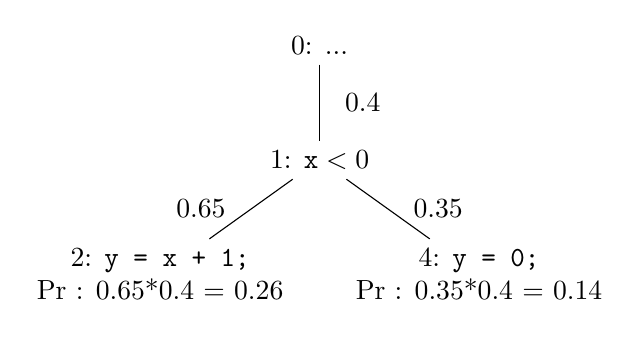
\begin{tikzpicture}[scale=0.7]
  \node {0: ...}
     child {
       node[xshift=0mm, yshift=-4mm] {1: $\mathtt{x} < 0$}
       child {
         node[xshift=-15mm, yshift=-4mm, align=center] {2: \texttt{y = x + 1;}\\
                                          Pr : 0.65*0.4 = 0.26}
         edge from parent node[left, xshift=-2mm] {$0.65$}
       }
       child {
         node[xshift=15mm, yshift=-4mm, align=center] {4: \texttt{y = 0;}\\
                                         Pr : 0.35*0.4 = 0.14}
         edge from parent node[right, xshift=2mm] {$0.35$}
       }
       edge from parent node[right, xshift=2mm] {$0.4$}
     };
\end{tikzpicture}
\end{center}
\vfill
This makes sense in some cases, e.g., \texttt{x = bernoulli(0.5);}
\vfill
\end{frame}

\begin{frame}[fragile]
\frametitle{Breaking down the PPA literature}
\vfill
Probabilistic program analyses can be broken down in several dimensions
\begin{itemize}
\item approximating $f$ vs. \textcolor{red}{approximating $Pr[p(X)]$ for some predicate $p$}
\item \textcolor{red}{approximating from above (below) vs. a ``close'' approximation}
\item \textcolor{red}{explicit choice probability} vs. implicit choice probability
\end{itemize}
\mbox{~}\\
A body of work makes the simplifying assumption that branch probabilities are given (this includes all work on probabilistic model checking)\\
\mbox{~}\\
Ramalingam (1996) generalized Kildall's framework to accumulate path probabilities\\
\mbox{~}\\
This is equivalent to PRISM's support for DTMCs --- see Kwiatkowska et al (2011)\\
\mbox{~}\\
Wachter and Zhang (2010), Esparza and Gaiser (2011), and Kwiatkowska et al (2011) apply predicate abstraction to data to scale probabilistic model checking to software
\mbox{~}\\
\vfill
\end{frame}

\begin{frame}[fragile]
\frametitle{Breaking down the PPA literature}
\vfill
Probabilistic program analyses can be broken down in several dimensions
\begin{itemize}
\item approximating $f$ vs. \textcolor{red}{approximating $Pr[p(X)]$ for some predicate $p$}
\item approximating from above (below) vs. \textcolor{red}{a ``close'' approximation}
\item explicit choice probability vs. \textcolor{red}{implicit choice probability}
\end{itemize}
\mbox{~}\\
Sankaranarayanan et al (2013) estimate the property probabilities using a path selection approach to drive symbolic execution\\
\mbox{~}\\
We developed probabilistic symbolic execution in a series of papers (2012-2015) that, novely, computes the conditional choice probabilities for branches along paths
\mbox{~}\\
\vfill
\end{frame}

\begin{frame}[fragile]
\frametitle{A simple example ...}
\begin{center}
\begin{lstlisting}
int classify(int a, int b, int c) {
  if (a<=0 || b<=0 || c<=0) return 4;
  int type=0;
  if (a==b) type+=1;
  if (a==c) type+=2;
  if (b==c) type+=3;
  if (type==0) {
    if (a+b<=c || b+c<=a || a+c>=b) type=4;
    else type=1;
    return type;
  }
  if (type>3) type=3;
  else if (type==1 && a+b>c) type=2;
  else if (type==2 && a+c>b) type=2;
  else if (type==3 && b+c>a) type=2;
  else type=4;
  return type;
}
\end{lstlisting}
\end{center}
\end{frame}

\newcommand{\Hilight}{\makebox[0pt][l]{\color{yellow}\rule[-0.45em]{\linewidth}{1.5em}}}
\begin{frame}[fragile]
\frametitle{A simple example ...}
\begin{center}
\begin{lstlisting}[escapechar=\%]
int classify(int a, int b, int c) {
  %\Hilight%if (a<=0 || b<=0 || c<=0) return 4;
  int type=0;
  if (a==b) type+=1;
  if (a==c) type+=2;
  if (b==c) type+=3;
  if (type==0) {
    if (a+b<=c || b+c<=a || a+c>=b) type=4;
    else type=1;
    return type;
  }
  if (type>3) type=3;
  else if (type==1 && a+b>c) type=2;
  else if (type==2 && a+c>b) type=2;
  else if (type==3 && b+c>a) type=2;
  else type=4;
  return type;
}
\end{lstlisting}
\end{center}
\end{frame}

\begin{frame}{Symbolic execution tree}
\begin{center}
\begin{tikzpicture}[scale=0.6]
  \node {\texttt{a$\le$0}}
     child {
       node[xshift=-7mm, yshift=3mm] {\colorbox{Green}{4}}
       edge from parent
     }
     child {
       node[xshift=5mm, yshift=3mm] {$b \le 0$}
       child {
         node[xshift=-7mm, yshift=3mm] {\colorbox{Green}{4}}
         edge from parent
       }
       child {
         node[xshift=5mm, yshift=3mm] {$c \le 0$}
         child {
           node[xshift=-7mm, yshift=3mm] {\colorbox{Green}{4}}
           edge from parent
         }
         child [color=white] {
           node[xshift=5mm, yshift=3mm] {$a=b$}
           child {
             node[xshift=-30mm, yshift=2mm] {$a=c$}
             child {
               node[xshift=-4mm, yshift=3mm] {$b=c$}
               child {
                 node[xshift=0mm, yshift=2mm] {}
                 edge from parent
               }
               child {
                 node[xshift=0mm, yshift=2mm] {}
                 edge from parent
               }
               edge from parent
             }
             child {
               node[xshift=4mm, yshift=3mm] {$b=c$}
               child {
                 node[xshift=-2mm, yshift=2mm] {}
                 edge from parent
               }
               child { 
                 node[xshift=0mm, yshift=2mm] {$a+b>c$}
                 child {
                   node[yshift=2mm] {}
                   edge from parent
                 }
                 child {
                   node[yshift=2mm] {}
                   edge from parent
                 }
                 edge from parent
               }
               edge from parent
             }
             edge from parent
           }
           child {
             node[xshift=10mm, yshift=2mm] {$a=c$}
             child {
               node[xshift=-13mm, yshift=3mm] {$b=c$}
               child {
                 node[xshift=-2mm, yshift=2mm] {}
                 edge from parent
               }
               child {
                 node[xshift=0mm, yshift=2mm] {$a+c>b$}
                 child {
                   node[yshift=2mm] {}
                   edge from parent
                 }
                 child {
                   node[yshift=2mm] {}
                   edge from parent
                 }
                 edge from parent
               }
               edge from parent
             }
             child {
               node[xshift=20mm, yshift=3mm] {$b=c$}
               child {
                 node[xshift=-15mm, yshift=2mm] {$b+c>a$}
                 child {
                   node[yshift=2mm] {}
                   edge from parent
                 }
                 child {
                   node[yshift=2mm] {}
                   edge from parent
                 }
                 edge from parent
               }
               child {
                 node[xshift=0mm, yshift=2mm] {$a+b \le c$}
                 child {
                   node[xshift=-5mm, yshift=2mm] {}
                   edge from parent
                 }
                 child {
                   node[xshift=5mm, yshift=2mm] {$b+c \le a$}
                   child {
                     node[xshift=-5mm, yshift=2mm] {}
                     edge from parent
                   }
                   child {
                     node[xshift=0mm, yshift=2mm] {$a+c \ge b$}
                     child {
                       node[yshift=2mm] {}
                       edge from parent
                     }
                     child {
                       node[yshift=2mm] {}
                       edge from parent
                     }
                     edge from parent
                   }
                   edge from parent
                 }
                 edge from parent
               }
               edge from parent
             }
             edge from parent
           }
           edge from parent
         }
         edge from parent
       }
       edge from parent
     };
\end{tikzpicture}
\end{center}
\end{frame}

\begin{frame}[fragile]
\frametitle{A simple example ...}
\begin{center}
\begin{lstlisting}[escapechar=\%]
int classify(int a, int b, int c) {
  if (a<=0 || b<=0 || c<=0) return 4;
  int type=0;
  %\Hilight%if (a==b) type+=1;
  %\Hilight%if (a==c) type+=2;
  %\Hilight%if (b==c) type+=3;
  if (type==0) {
    if (a+b<=c || b+c<=a || a+c>=b) type=4;
    else type=1;
    return type;
  }
  if (type>3) type=3;
  else if (type==1 && a+b>c) type=2;
  else if (type==2 && a+c>b) type=2;
  else if (type==3 && b+c>a) type=2;
  else type=4;
  return type;
}
\end{lstlisting}
\end{center}
\end{frame}

\begin{frame}{Symbolic execution tree}
\begin{center}
\begin{tikzpicture}[scale=0.6]
  \node {\texttt{a$\le$0}}
     child {
       node[xshift=-7mm, yshift=3mm] {\colorbox{Green}{4}}
       edge from parent
     }
     child {
       node[xshift=5mm, yshift=3mm] {$b \le 0$}
       child {
         node[xshift=-7mm, yshift=3mm] {\colorbox{Green}{4}}
         edge from parent
       }
       child {
         node[xshift=5mm, yshift=3mm] {$c \le 0$}
         child {
           node[xshift=-7mm, yshift=3mm] {\colorbox{Green}{4}}
           edge from parent
         }
         child {
           node[xshift=5mm, yshift=3mm] {$a=b$}
           child {
             node[xshift=-30mm, yshift=2mm] {$a=c$}
             child {
               node[xshift=-4mm, yshift=3mm] {$b=c$}
               child [color=white] {
                 node[xshift=0mm, yshift=2mm] {}
                 edge from parent
               }
               child [color=white] {
                 node[xshift=0mm, yshift=2mm] {}
                 edge from parent
               }
               edge from parent
             }
             child {
               node[xshift=4mm, yshift=3mm] {$b=c$}
               child [color=white] {
                 node[xshift=-2mm, yshift=2mm] {}
                 edge from parent
               }
               child [color=white] { 
                 node[xshift=0mm, yshift=2mm] {$a+b>c$}
                 child {
                   node[yshift=2mm] {}
                   edge from parent
                 }
                 child {
                   node[yshift=2mm] {}
                   edge from parent
                 }
                 edge from parent
               }
               edge from parent
             }
             edge from parent
           }
           child {
             node[xshift=10mm, yshift=2mm] {$a=c$}
             child {
               node[xshift=-13mm, yshift=3mm] {$b=c$}
               child [color=white] {
                 node[xshift=-2mm, yshift=2mm] {}
                 edge from parent
               }
               child [color=white] {
                 node[xshift=0mm, yshift=2mm] {$a+c>b$}
                 child {
                   node[yshift=2mm] {}
                   edge from parent
                 }
                 child {
                   node[yshift=2mm] {}
                   edge from parent
                 }
                 edge from parent
               }
               edge from parent
             }
             child {
               node[xshift=20mm, yshift=3mm] {$b=c$}
               child [color=white] {
                 node[xshift=-15mm, yshift=2mm] {$b+c>a$}
                 child {
                   node[yshift=2mm] {}
                   edge from parent
                 }
                 child {
                   node[yshift=2mm] {}
                   edge from parent
                 }
                 edge from parent
               }
               child [color=white] {
                 node[xshift=0mm, yshift=2mm] {$a+b \le c$}
                 child {
                   node[xshift=-5mm, yshift=2mm] {}
                   edge from parent
                 }
                 child {
                   node[xshift=5mm, yshift=2mm] {$b+c \le a$}
                   child {
                     node[xshift=-5mm, yshift=2mm] {}
                     edge from parent
                   }
                   child {
                     node[xshift=0mm, yshift=2mm] {$a+c \ge b$}
                     child {
                       node[yshift=2mm] {}
                       edge from parent
                     }
                     child {
                       node[yshift=2mm] {}
                       edge from parent
                     }
                     edge from parent
                   }
                   edge from parent
                 }
                 edge from parent
               }
               edge from parent
             }
             edge from parent
           }
           edge from parent
         }
         edge from parent
       }
       edge from parent
     };
\end{tikzpicture}
\end{center}
\end{frame}

\begin{frame}[fragile]
\frametitle{A simple example ...}
\begin{center}
\begin{lstlisting}[escapechar=\%]
int classify(int a, int b, int c) {
  if (a<=0 || b<=0 || c<=0) return 4;
  int type=0;
  if (a==b) type+=1;
  if (a==c) type+=2;
  if (b==c) type+=3;
  if (type==0) {
    if (a+b<=c || b+c<=a || a+c>=b) type=4;
    else type=1;
    return type;
  }
  %\Hilight%if (type>3) type=3;
  %\Hilight%else if (type==1 && a+b>c) type=2;
  %\Hilight%else if (type==2 && a+c>b) type=2;
  %\Hilight%else if (type==3 && b+c>a) type=2;
  %\Hilight%else type=4;
  return type;
}
\end{lstlisting}
\end{center}
\end{frame}

\begin{frame}{Symbolic execution tree}
\begin{center}
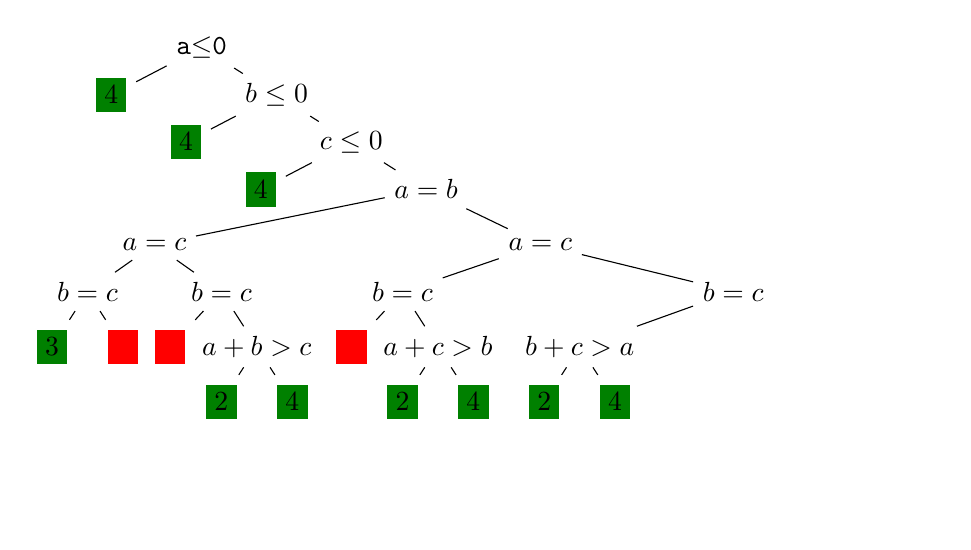
\begin{tikzpicture}[scale=0.6]
  \node {\texttt{a$\le$0}}
     child [color=black] {
       node[xshift=-7mm, yshift=3mm] {\colorbox{Green}{4}}
       edge from parent
     }
     child [color=black] {
       node[xshift=5mm, yshift=3mm] {$b \le 0$}
       child {
         node[xshift=-7mm, yshift=3mm] {\colorbox{Green}{4}}
         edge from parent
       }
       child {
         node[xshift=5mm, yshift=3mm] {$c \le 0$}
         child {
           node[xshift=-7mm, yshift=3mm] {\colorbox{Green}{4}}
           edge from parent
         }
         child {
           node[xshift=5mm, yshift=3mm] {$a=b$}
           child {
             node[xshift=-30mm, yshift=2mm] {$a=c$}
             child {
               node[xshift=-4mm, yshift=3mm] {$b=c$}
               child {
                 node[xshift=0mm, yshift=2mm] {\colorbox{Green}{3}}
                 edge from parent
               }
               child {
                 node[xshift=0mm, yshift=2mm] {\colorbox{Red}{\textcolor{Red}{3}}}
                 edge from parent
               }
               edge from parent
             }
             child {
               node[xshift=4mm, yshift=3mm] {$b=c$}
               child {
                 node[xshift=-2mm, yshift=2mm] {\colorbox{Red}{\textcolor{Red}{3}}}
                 edge from parent
               }
               child { 
                 node[xshift=0mm, yshift=2mm] {$a+b>c$}
                 child {
                   node[yshift=2mm] {\colorbox{Green}{2}}
                   edge from parent
                 }
                 child {
                   node[yshift=2mm] {\colorbox{Green}{4}}
                   edge from parent
                 }
                 edge from parent
               }
               edge from parent
             }
             edge from parent
           }
           child {
             node[xshift=10mm, yshift=2mm] {$a=c$}
             child {
               node[xshift=-13mm, yshift=3mm] {$b=c$}
               child {
                 node[xshift=-2mm, yshift=2mm] {\colorbox{Red}{\textcolor{Red}{3}}}
                 edge from parent
               }
               child {
                 node[xshift=0mm, yshift=2mm] {$a+c>b$}
                 child {
                   node[yshift=2mm] {\colorbox{Green}{2}}
                   edge from parent
                 }
                 child {
                   node[yshift=2mm] {\colorbox{Green}{4}}
                   edge from parent
                 }
                 edge from parent
               }
               edge from parent
             }
             child {
               node[xshift=20mm, yshift=3mm] {$b=c$}
               child {
                 node[xshift=-15mm, yshift=2mm] {$b+c>a$}
                 child {
                   node[yshift=2mm] {\colorbox{Green}{2}}
                   edge from parent
                 }
                 child {
                   node[yshift=2mm] {\colorbox{Green}{4}}
                   edge from parent
                 }
                 edge from parent
               }
               child [color=white] {
                 node[xshift=0mm, yshift=2mm] {$a+b \le c$}
                 child {
                   node[xshift=-5mm, yshift=2mm] {}
                   edge from parent
                 }
                 child {
                   node[xshift=5mm, yshift=2mm] {$b+c \le a$}
                   child {
                     node[xshift=-5mm, yshift=2mm] {}
                     edge from parent
                   }
                   child {
                     node[xshift=0mm, yshift=2mm] {$a+c \ge b$}
                     child {
                       node[yshift=2mm] {}
                       edge from parent
                     }
                     child {
                       node[yshift=2mm] {}
                       edge from parent
                     }
                     edge from parent
                   }
                   edge from parent
                 }
                 edge from parent
               }
               edge from parent
             }
             edge from parent
           }
           edge from parent
         }
         edge from parent
       }
       edge from parent
     };
\end{tikzpicture}
\end{center}
\end{frame}

\begin{frame}[fragile]
\frametitle{A simple example ...}
\begin{center}
\begin{lstlisting}[escapechar=\%]
int classify(int a, int b, int c) {
  if (a<=0 || b<=0 || c<=0) return 4;
  int type=0;
  if (a==b) type+=1;
  if (a==c) type+=2;
  if (b==c) type+=3;
  if (type==0) {
    %\Hilight%if (a+b<=c || b+c<=a || a+c>=b) type=4;
    %\Hilight%else type=1;
    %\Hilight%return type;
  }
  if (type>3) type=3;
  else if (type==1 && a+b>c) type=2;
  else if (type==2 && a+c>b) type=2;
  else if (type==3 && b+c>a) type=2;
  else type=4;
  return type;
}
\end{lstlisting}
\end{center}
\end{frame}

\begin{frame}{Symbolic execution tree}
\begin{center}
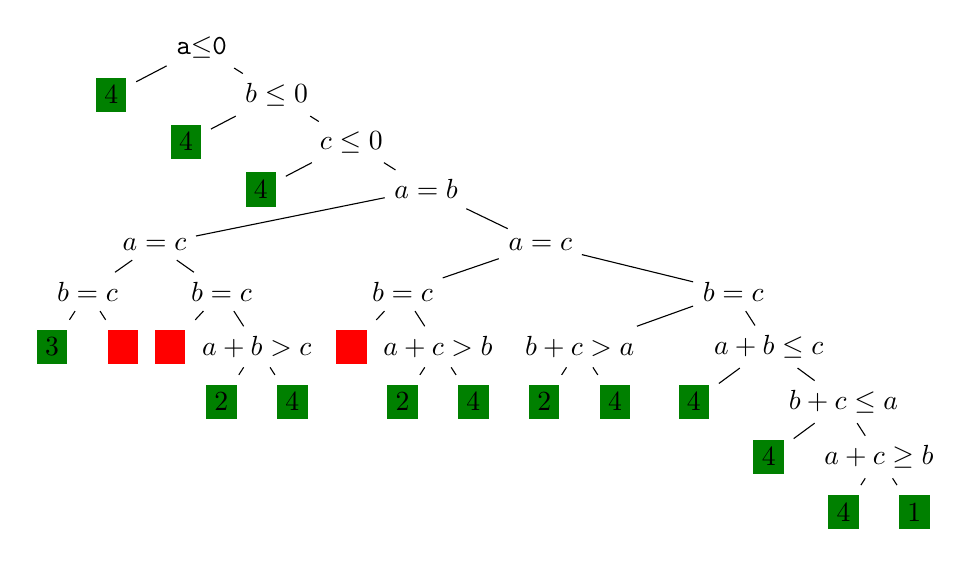
\begin{tikzpicture}[scale=0.6]
  \node {\texttt{a$\le$0}}
     child [color=black] {
       node[xshift=-7mm, yshift=3mm] {\colorbox{Green}{4}}
       edge from parent
     }
     child [color=black] {
       node[xshift=5mm, yshift=3mm] {$b \le 0$}
       child {
         node[xshift=-7mm, yshift=3mm] {\colorbox{Green}{4}}
         edge from parent
       }
       child {
         node[xshift=5mm, yshift=3mm] {$c \le 0$}
         child {
           node[xshift=-7mm, yshift=3mm] {\colorbox{Green}{4}}
           edge from parent
         }
         child {
           node[xshift=5mm, yshift=3mm] {$a=b$}
           child {
             node[xshift=-30mm, yshift=2mm] {$a=c$}
             child {
               node[xshift=-4mm, yshift=3mm] {$b=c$}
               child {
                 node[xshift=0mm, yshift=2mm] {\colorbox{Green}{3}}
                 edge from parent
               }
               child {
                 node[xshift=0mm, yshift=2mm] {\colorbox{Red}{\textcolor{Red}{3}}}
                 edge from parent
               }
               edge from parent
             }
             child {
               node[xshift=4mm, yshift=3mm] {$b=c$}
               child {
                 node[xshift=-2mm, yshift=2mm] {\colorbox{Red}{\textcolor{Red}{3}}}
                 edge from parent
               }
               child { 
                 node[xshift=0mm, yshift=2mm] {$a+b>c$}
                 child {
                   node[yshift=2mm] {\colorbox{Green}{2}}
                   edge from parent
                 }
                 child {
                   node[yshift=2mm] {\colorbox{Green}{4}}
                   edge from parent
                 }
                 edge from parent
               }
               edge from parent
             }
             edge from parent
           }
           child {
             node[xshift=10mm, yshift=2mm] {$a=c$}
             child {
               node[xshift=-13mm, yshift=3mm] {$b=c$}
               child {
                 node[xshift=-2mm, yshift=2mm] {\colorbox{Red}{\textcolor{Red}{3}}}
                 edge from parent
               }
               child {
                 node[xshift=0mm, yshift=2mm] {$a+c>b$}
                 child {
                   node[yshift=2mm] {\colorbox{Green}{2}}
                   edge from parent
                 }
                 child {
                   node[yshift=2mm] {\colorbox{Green}{4}}
                   edge from parent
                 }
                 edge from parent
               }
               edge from parent
             }
             child {
               node[xshift=20mm, yshift=3mm] {$b=c$}
               child {
                 node[xshift=-15mm, yshift=2mm] {$b+c>a$}
                 child {
                   node[yshift=2mm] {\colorbox{Green}{2}}
                   edge from parent
                 }
                 child {
                   node[yshift=2mm] {\colorbox{Green}{4}}
                   edge from parent
                 }
                 edge from parent
               }
               child {
                 node[xshift=0mm, yshift=2mm] {$a+b \le c$}
                 child {
                   node[xshift=-5mm, yshift=2mm] {\colorbox{Green}{4}}
                   edge from parent
                 }
                 child {
                   node[xshift=5mm, yshift=2mm] {$b+c \le a$}
                   child {
                     node[xshift=-5mm, yshift=2mm] {\colorbox{Green}{4}}
                     edge from parent
                   }
                   child {
                     node[xshift=0mm, yshift=2mm] {$a+c \ge b$}
                     child {
                       node[yshift=2mm] {\colorbox{Green}{4}}
                       edge from parent
                     }
                     child {
                       node[yshift=2mm] {\colorbox{Green}{1}}
                       edge from parent
                     }
                     edge from parent
                   }
                   edge from parent
                 }
                 edge from parent
               }
               edge from parent
             }
             edge from parent
           }
           edge from parent
         }
         edge from parent
       }
       edge from parent
     };
\end{tikzpicture}
\end{center}
\end{frame}

\begin{frame}{Some observations}
\vfill
\begin{itemize}
\item There are 14 distinct paths (Green): from 1 to 9 branches
\vfill
\item 1 path returns ``scalene'' (1); 3 return ``isoscelese'' (2); and 1 returns ``equilateral'' (3)
\vfill
\item 3 paths are pruned because constraints are unsat (Red)
\vfill
\item Interesting symmetries are involved in the ``isoscelese'' and unsat cases
\end{itemize}
\vfill
\end{frame}


\begin{frame}{Adding probabilities}
\vfill
The key insight here is to shift from using SAT queries to \textit{counting} queries ($\#$)
\begin{itemize}
\item cost ranges from fast, e.g., $\#([a,b])$, to exponential
\item cost-effective $\#$ procedures may not be available
\item use statistical estimators when necessary
\end{itemize}
\vfill
Probability estimates can be very precise for state space that is analyzed
\begin{itemize}
\item computes an underapproximation of state probabilities
\item unanalyzed state space can be quantified
\end{itemize}
\vfill
Numerous layers of optimization required to make it efficient
\begin{itemize}
\item due to optimizations initial versions ran faster then classic symbolic execution (backpatched compatible optimizations)
\item still limited to programs with 10s of thousands of SLOC
\end{itemize}
\vfill
\end{frame}

\begin{frame}{Assume \texttt{int}s are drawn uniformly from $[-1000,1000]$}
\begin{center}
\pgfdeclarelayer{foreground}
\pgfsetlayers{main,foreground}
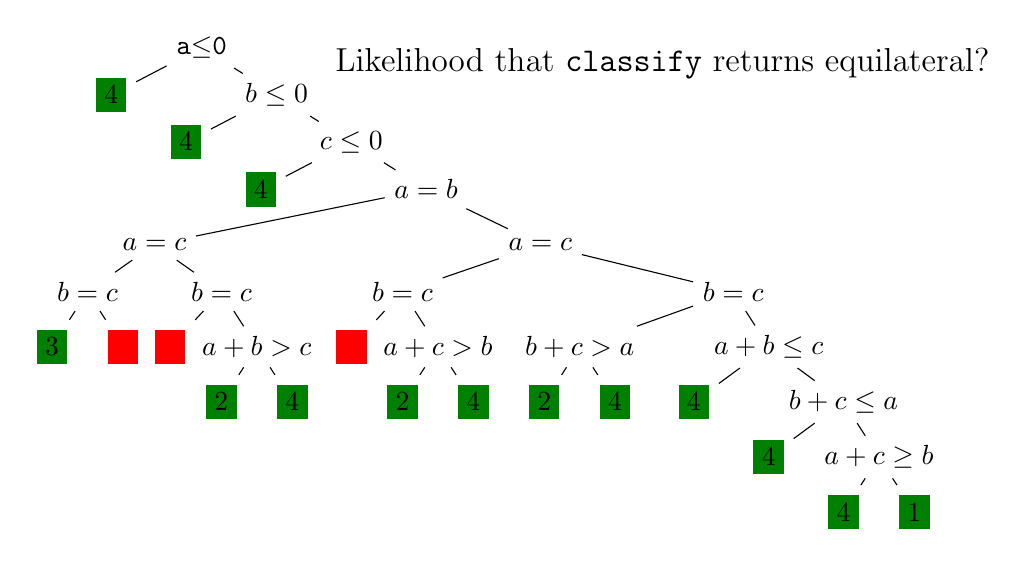
\begin{tikzpicture}[scale=0.6]
  \node {\texttt{a$\le$0}}
     child [color=black] {
       node[xshift=-7mm, yshift=3mm] {\colorbox{Green}{4}}
       edge from parent
     }
     child [color=black] {
       node[xshift=5mm, yshift=3mm] {$b \le 0$}
       child {
         node[xshift=-7mm, yshift=3mm] {\colorbox{Green}{4}}
         edge from parent
       }
       child {
         node[xshift=5mm, yshift=3mm] {$c \le 0$}
         child {
           node[xshift=-7mm, yshift=3mm] {\colorbox{Green}{4}}
           edge from parent
         }
         child {
           node[name=reference, xshift=5mm, yshift=3mm] {$a=b$}
           child {
             node[xshift=-30mm, yshift=2mm] {$a=c$}
             child {
               node[xshift=-4mm, yshift=3mm] {$b=c$}
               child {
                 node[xshift=0mm, yshift=2mm] {\colorbox{Green}{3}}
                 edge from parent
               }
               child {
                 node[xshift=0mm, yshift=2mm] {\colorbox{Red}{\textcolor{Red}{3}}}
                 edge from parent
               }
               edge from parent
             }
             child {
               node[xshift=4mm, yshift=3mm] {$b=c$}
               child {
                 node[xshift=-2mm, yshift=2mm] {\colorbox{Red}{\textcolor{Red}{3}}}
                 edge from parent
               }
               child { 
                 node[xshift=0mm, yshift=2mm] {$a+b>c$}
                 child {
                   node[yshift=2mm] {\colorbox{Green}{2}}
                   edge from parent
                 }
                 child {
                   node[yshift=2mm] {\colorbox{Green}{4}}
                   edge from parent
                 }
                 edge from parent
               }
               edge from parent
             }
             edge from parent
           }
           child {
             node[xshift=10mm, yshift=2mm] {$a=c$}
             child {
               node[xshift=-13mm, yshift=3mm] {$b=c$}
               child {
                 node[xshift=-2mm, yshift=2mm] {\colorbox{Red}{\textcolor{Red}{3}}}
                 edge from parent
               }
               child {
                 node[xshift=0mm, yshift=2mm] {$a+c>b$}
                 child {
                   node[yshift=2mm] {\colorbox{Green}{2}}
                   edge from parent
                 }
                 child {
                   node[yshift=2mm] {\colorbox{Green}{4}}
                   edge from parent
                 }
                 edge from parent
               }
               edge from parent
             }
             child {
               node[xshift=20mm, yshift=3mm] {$b=c$}
               child {
                 node[xshift=-15mm, yshift=2mm] {$b+c>a$}
                 child {
                   node[yshift=2mm] {\colorbox{Green}{2}}
                   edge from parent
                 }
                 child {
                   node[yshift=2mm] {\colorbox{Green}{4}}
                   edge from parent
                 }
                 edge from parent
               }
               child {
                 node[xshift=0mm, yshift=2mm] {$a+b \le c$}
                 child {
                   node[xshift=-5mm, yshift=2mm] {\colorbox{Green}{4}}
                   edge from parent
                 }
                 child {
                   node[xshift=5mm, yshift=2mm] {$b+c \le a$}
                   child {
                     node[xshift=-5mm, yshift=2mm] {\colorbox{Green}{4}}
                     edge from parent
                   }
                   child {
                     node[xshift=0mm, yshift=2mm] {$a+c \ge b$}
                     child {
                       node[yshift=2mm] {\colorbox{Green}{4}}
                       edge from parent
                     }
                     child {
                       node[yshift=2mm] {\colorbox{Green}{1}}
                       edge from parent
                     }
                     edge from parent
                   }
                   edge from parent
                 }
                 edge from parent
               }
               edge from parent
             }
             edge from parent
           }
           edge from parent
         }
         edge from parent
       }
       edge from parent
     };

   \begin{pgfonlayer}{foreground}
      \node[name=first, xshift=30mm, yshift=6mm, above of=reference] 
         {\large Likelihood that \texttt{classify} returns equilateral?}; 
   \end{pgfonlayer}

\end{tikzpicture}
\end{center}
\end{frame}

\begin{frame}{Assume \texttt{int}s are drawn uniformly from $[-1000,1000]$}
\begin{center}
\pgfdeclarelayer{foreground}
\pgfsetlayers{main,foreground}
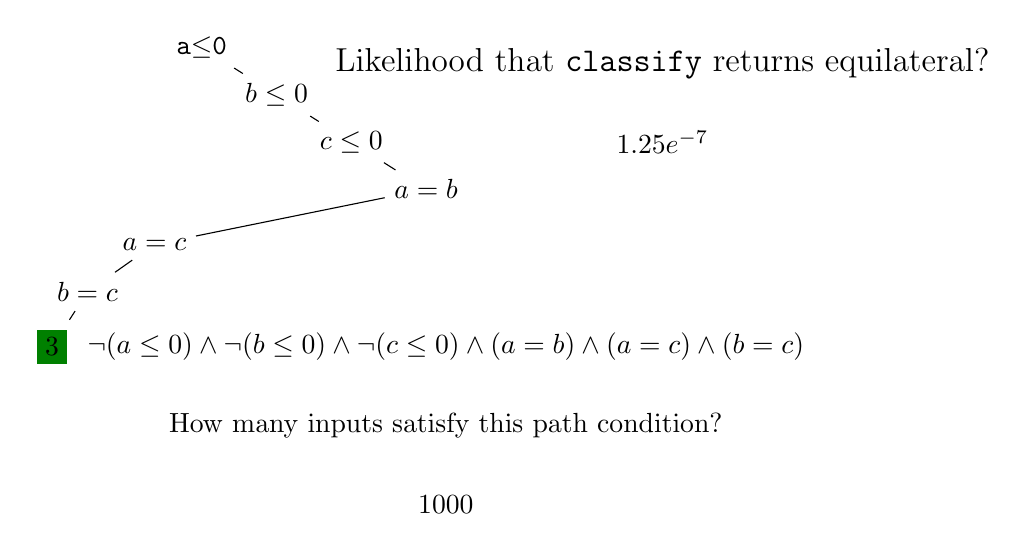
\begin{tikzpicture}[scale=0.6]
  \node {\texttt{a$\le$0}}
     child [color=white] {
       node[xshift=-7mm, yshift=3mm] {}
       edge from parent
     }
     child {
       node[xshift=5mm, yshift=3mm] {$b \le 0$}
       child [color=white] {
         node[xshift=-7mm, yshift=3mm] {}
         edge from parent
       }
       child {
         node[xshift=5mm, yshift=3mm] {$c \le 0$}
         child [color=white] {
           node[xshift=-7mm, yshift=3mm] {}
           edge from parent
         }
         child {
           node[name=reference, xshift=5mm, yshift=3mm] {$a=b$}
           child {
             node[xshift=-30mm, yshift=2mm] {$a=c$}
             child {
               node[xshift=-4mm, yshift=3mm] {$b=c$}
               child {
                 node[name=ref2, xshift=0mm, yshift=2mm] {\colorbox{Green}{3}}
                 edge from parent
               }
               child [color=white]{
                 node[xshift=0mm, yshift=2mm] {}
                 edge from parent
               }
               edge from parent
             }
             child [color=white] {
               node[xshift=4mm, yshift=3mm] {$b=c$}
               child {
                 node[xshift=-2mm, yshift=2mm] {}
                 edge from parent
               }
               child { 
                 node[xshift=0mm, yshift=2mm] {$a+b>c$}
                 child {
                   node[yshift=2mm] {}
                   edge from parent
                 }
                 child {
                   node[yshift=2mm] {}
                   edge from parent
                 }
                 edge from parent
               }
               edge from parent
             }
             edge from parent
           }
           child [color=white] {
             node[xshift=10mm, yshift=2mm] {$a=c$}
             child [color=white] {
               node[xshift=-13mm, yshift=3mm] {$b=c$}
               child {
                 node[xshift=-2mm, yshift=2mm] {}
                 edge from parent
               }
               child {
                 node[xshift=0mm, yshift=2mm] {$a+c>b$}
                 child {
                   node[yshift=2mm] {}
                   edge from parent
                 }
                 child {
                   node[yshift=2mm] {}
                   edge from parent
                 }
                 edge from parent
               }
               edge from parent
             }
             child {
               node[xshift=20mm, yshift=3mm] {$b=c$}
               child [color=white] {
                 node[xshift=-15mm, yshift=2mm] {$b+c>a$}
                 child {
                   node[yshift=2mm] {}
                   edge from parent
                 }
                 child {
                   node[yshift=2mm] {}
                   edge from parent
                 }
                 edge from parent
               }
               child {
                 node[xshift=0mm, yshift=2mm] {$a+b \le c$}
                 child {
                   node[xshift=-5mm, yshift=2mm] {}
                   edge from parent
                 }
                 child {
                   node[xshift=5mm, yshift=2mm] {$b+c \le a$}
                   child {
                     node[xshift=-5mm, yshift=2mm] {}
                     edge from parent
                   }
                   child {
                     node[xshift=0mm, yshift=2mm] {$a+c \ge b$}
                     child {
                       node[yshift=2mm] {}
                       edge from parent
                     }
                     child {
                       node[yshift=2mm] {}
                       edge from parent
                     }
                     edge from parent
                   }
                   edge from parent
                 }
                 edge from parent
               }
               edge from parent
             }
             edge from parent
           }
           edge from parent
         }
         edge from parent
       }
       edge from parent
     };

   \begin{pgfonlayer}{foreground}
      \node[name=first, xshift=30mm, yshift=6mm, above of=reference] 
         {\large Likelihood that \texttt{classify} returns equilateral?}; 
       \pause
       \node[name=pc, right of=ref2, xshift=40mm] 
          {$\neg(a\le0) \wedge \neg(b\le0) \wedge \neg(c\le0) \wedge (a=b) \wedge (a=c) \wedge (b=c)$}; 
       \pause
       \node[name=question, below of=pc] 
          {How many inputs satisfy this path condition?};
       \pause
       \node[name=answer, below of=question] 
          {1000};
       \pause
       \node[name=firstanswer, below of=first] 
          {$1.25e^{-7}$};
   \end{pgfonlayer}

\end{tikzpicture}
\end{center}
\end{frame}

\begin{frame}{Assume \texttt{int}s are drawn uniformly from $[-1000,1000]$}
\begin{center}
\pgfdeclarelayer{foreground}
\pgfsetlayers{main,foreground}
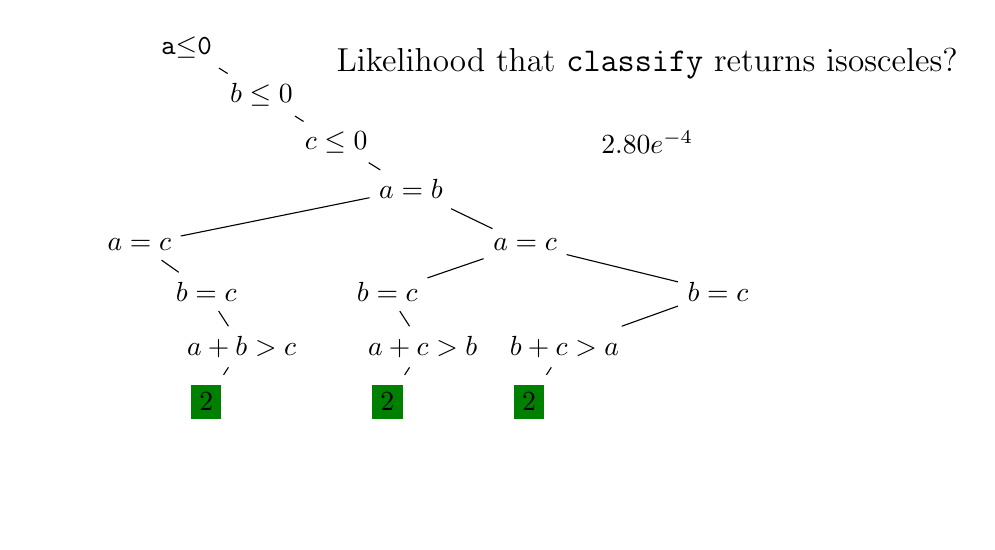
\begin{tikzpicture}[scale=0.6]
  \node {\texttt{a$\le$0}}
     child [color=white] {
       node[xshift=-7mm, yshift=3mm] {}
       edge from parent
     }
     child [color=black] {
       node[xshift=5mm, yshift=3mm] {$b \le 0$}
       child [color=white] {
         node[xshift=-7mm, yshift=3mm] {}
         edge from parent
       }
       child {
         node[xshift=5mm, yshift=3mm] {$c \le 0$}
         child [color=white] {
           node[xshift=-7mm, yshift=3mm] {}
           edge from parent
         }
         child {
           node[name=reference, xshift=5mm, yshift=3mm] {$a=b$}
           child {
             node[xshift=-30mm, yshift=2mm] {$a=c$}
             child [color=white] {
               node[xshift=-4mm, yshift=3mm] {$b=c$}
               child {
                 node[xshift=0mm, yshift=2mm] {}
                 edge from parent
               }
               child {
                 node[xshift=0mm, yshift=2mm] {}
                 edge from parent
               }
               edge from parent
             }
             child {
               node[xshift=4mm, yshift=3mm] {$b=c$}
               child [color=white] {
                 node[xshift=-2mm, yshift=2mm] {}
                 edge from parent
               }
               child { 
                 node[xshift=0mm, yshift=2mm] {$a+b>c$}
                 child {
                   node[yshift=2mm] {\colorbox{Green}{2}}
                   edge from parent
                 }
                 child [color=white] {
                   node[yshift=2mm] {}
                   edge from parent
                 }
                 edge from parent
               }
               edge from parent
             }
             edge from parent
           }
           child {
             node[xshift=10mm, yshift=2mm] {$a=c$}
             child {
               node[xshift=-13mm, yshift=3mm] {$b=c$}
               child [color=white] {
                 node[xshift=-2mm, yshift=2mm] {}
                 edge from parent
               }
               child {
                 node[xshift=0mm, yshift=2mm] {$a+c>b$}
                 child {
                   node[yshift=2mm] {\colorbox{Green}{2}}
                   edge from parent
                 }
                 child [color=white] {
                   node[yshift=2mm] {}
                   edge from parent
                 }
                 edge from parent
               }
               edge from parent
             }
             child {
               node[xshift=20mm, yshift=3mm] {$b=c$}
               child {
                 node[xshift=-15mm, yshift=2mm] {$b+c>a$}
                 child {
                   node[yshift=2mm] {\colorbox{Green}{2}}
                   edge from parent
                 }
                 child [color=white] {
                   node[yshift=2mm] {}
                   edge from parent
                 }
                 edge from parent
               }
               child [color=white] {
                 node[xshift=0mm, yshift=2mm] {$a+b \le c$}
                 child {
                   node[xshift=-5mm, yshift=2mm] {}
                   edge from parent
                 }
                 child {
                   node[xshift=5mm, yshift=2mm] {$b+c \le a$}
                   child {
                     node[xshift=-5mm, yshift=2mm] {}
                     edge from parent
                   }
                   child {
                     node[xshift=0mm, yshift=2mm] {$a+c \ge b$}
                     child {
                       node[yshift=2mm] {}
                       edge from parent
                     }
                     child {
                       node[yshift=2mm] {}
                       edge from parent
                     }
                     edge from parent
                   }
                   edge from parent
                 }
                 edge from parent
               }
               edge from parent
             }
             edge from parent
           }
           edge from parent
         }
         edge from parent
       }
       edge from parent
     };

   \begin{pgfonlayer}{foreground}
      \node[name=first, xshift=30mm, yshift=6mm, above of=reference] 
         {\large Likelihood that \texttt{classify} returns isosceles?}; \pause
      \node[name=first, below of=first] 
         {$2.80e^{-4}$}; 
   \end{pgfonlayer}

\end{tikzpicture}
\end{center}
\end{frame}

\begin{frame}{Some observations}
\vfill
\begin{itemize}
\item You may be able to calculate these probabilities because you know about triangles.
\pause
\vfill
\item We want to calculate the probability that a program's execution ...
\begin{itemize}
\item returns a value, reaches a statement, ...
\end{itemize}
\vfill
\pause
\item Adapting symbolic execution to perform these computations involves ...
\begin{itemize}
\item calculating the paths of interest
\item calculating the probability of taking those paths
\item combining those probabilities appropriately
\end{itemize}
\end{itemize}
\vfill
\end{frame}

\begin{frame}{Probabilistic symbolic execution algorithm} 
\vfill
\begin{algorithm}[H]
\small
\caption{$\x{probSymEx}(l,m,pc,$\colorbox{yellow}{$Pr_{pc}$}$)$}
\begin{algorithmic}
 \IF{$\x{stoppingPath}(pc)$}
 \RETURN $pc$
 \ENDIF

 \WHILE{$\neg branch(l)$}
   \STATE $m \gets op(l)(m)$
   \STATE $l \gets succ(l)$
 \ENDWHILE

 \STATE $c \gets \x{cond}(l)(m)$

 \STATE \colorbox{yellow}{$pc' \gets \x{slice}(pc, c)$}
 \STATE \colorbox{yellow}{$Pr_c \gets \x{prob}(pc' \land c) /\x{prob}(pc')$}

 \IF{\colorbox{yellow}{$Pr_c > 0$}}
   \STATE $\x{probSymEx}(succ_t(l), pc \wedge c, m,$\colorbox{yellow}{$Pr_{pc}*Pr_c$}$)$
 \ENDIF

 \IF{\colorbox{yellow}{$Pr_c < 1$}}
   \STATE $\x{probSymEx}(succ_f(l), pc \wedge \neg c, m,$\colorbox{yellow}{$Pr_{pc}*(1-Pr_c)$}$)$
 \ENDIF
\end{algorithmic}
\end{algorithm}
\end{frame}

\begin{frame}{Key algorithmic features (Geldenhuys et al ISSTA'12)}
\vfill
Slicing the path condition, i.e., $\x{slice}(pc,c)$
\begin{itemize}
\item reduces formula size which reduces cost of $\x{prob}(\cdot)$
\item exposes opportunities for reusing computation in $\x{prob}(\cdot)$
\end{itemize}
\pause
\vfill
Calculating the conditional probability $Pr_c$ of $c$
\begin{itemize}
\item requires model counting of path condition
\item determines satisfiability of branches, i.e., $Pr_c > 0 \implies SAT(pc \wedge c)$
\item allows inference of off-branch probability, i.e., $Pr_{pc}*(1-Pr_c)$
\item depth-first nature of symbolic execution ensures that $prob(pc')$ will be reused
\item slicing assures independence in computing $Pr_c$, i.e., $pc-pc'$ factored out
\end{itemize}
\pause
\vfill
This allows the algorithm to compute path probabilities cost-effectively.
\vfill
\end{frame}


%% in the following include the probabilities
%%   - Cyan ones are inferred (negated branch)
%%   - Orange ones are computed from reused prob(.) calls

\begin{frame}{Probabilistic symbolic execution tree}
\begin{center}
\pgfdeclarelayer{foreground}
\pgfsetlayers{main,foreground}
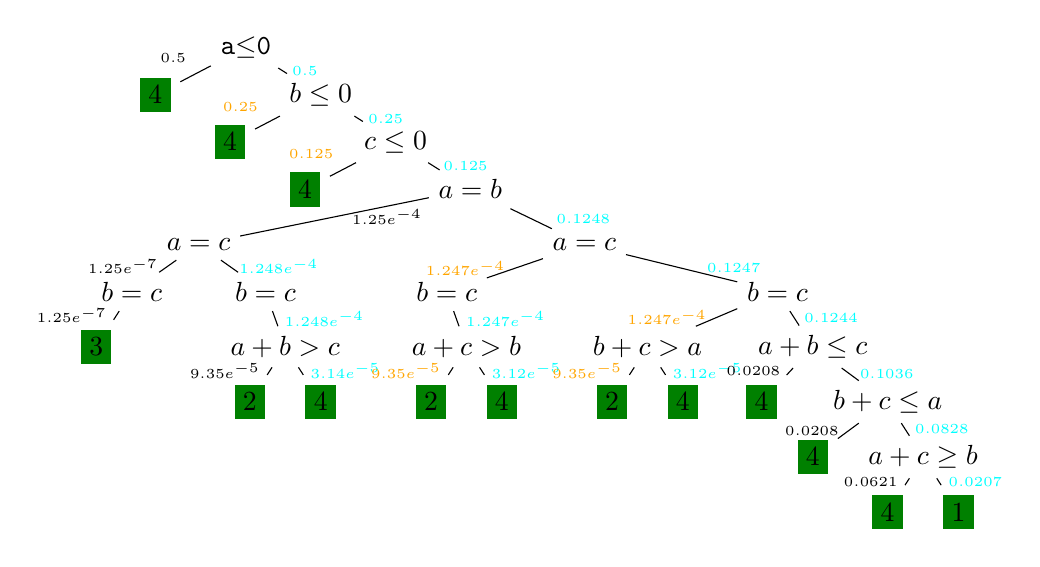
\begin{tikzpicture}[scale=0.6]
  \node {\texttt{a$\le$0}}
     child [color=black] {
       node[xshift=-7mm, yshift=3mm] {\colorbox{Green}{4}}
       edge from parent
       node[left, yshift=2mm] {\tiny $0.5$}
     }
     child [color=black] {
       node[xshift=5mm, yshift=3mm] {$b \le 0$}
       child {
         node[xshift=-7mm, yshift=3mm] {\colorbox{Green}{4}}
         edge from parent
         node[left, yshift=2mm] {\tiny \color{Orange}{$0.25$}}
       }
       child {
         node[xshift=5mm, yshift=3mm] {$c \le 0$}
         child {
           node[xshift=-7mm, yshift=3mm] {\colorbox{Green}{4}}
           edge from parent
           node[left, yshift=2mm] {\tiny \color{Orange}{$0.125$}}
         }
         child {
           node[xshift=5mm, yshift=3mm] {$a=b$}
           child {
             node[xshift=-30mm, yshift=2mm] {$a=c$}
             child {
               node[xshift=-4mm, yshift=3mm] {$b=c$}
               child {
                 node[xshift=0mm, yshift=2mm] {\colorbox{Green}{3}}
                 edge from parent
                 node[left] {\tiny $1.25e^{-7}$}
               }
               child [color=white] {
                 node[xshift=0mm, yshift=2mm] {\colorbox{white}{\textcolor{white}{3}}}
                 edge from parent
               }
               edge from parent
               node[left] {\tiny $1.25e^{-7}$}
             }
             child {
               node[xshift=4mm, yshift=3mm] {$b=c$}
               child [color=white] {
                 node[xshift=-2mm, yshift=2mm] {\colorbox{white}{\textcolor{white}{3}}}
                 edge from parent
               }
               child { 
                 node[xshift=-2mm, yshift=2mm] {$a+b>c$}
                 child {
                   node[yshift=2mm] {\colorbox{Green}{2}}
                   edge from parent
                   node[left] {\tiny $9.35e^{-5}$}
                 }
                 child {
                   node[yshift=2mm] {\colorbox{Green}{4}}
                   edge from parent
                   node[right] {\tiny \color{Cyan}{$3.14e^{-5}$}}
                 }
                 edge from parent
                 node[right] {\tiny \color{Cyan}{$1.248e^{-4}$}}
               }
               edge from parent
               node[right] {\tiny \color{Cyan}{$1.248e^{-4}$}}
             }
             edge from parent
             node[right, xshift=1mm] {\tiny {$1.25e^{-4}$}}
           }
           child {
             node[xshift=10mm, yshift=2mm] {$a=c$}
             child {
               node[xshift=-13mm, yshift=3mm] {$b=c$}
               child [color=white] {
                 node[xshift=-2mm, yshift=2mm] {\colorbox{white}{\textcolor{white}{3}}}
                 edge from parent
               }
               child {
                 node[xshift=-2mm, yshift=2mm] {$a+c>b$}
                 child {
                   node[yshift=2mm] {\colorbox{Green}{2}}
                   edge from parent
                   node[left] {\tiny \color{Orange}{$9.35e^{-5}$}}
                 }
                 child {
                   node[yshift=2mm] {\colorbox{Green}{4}}
                   edge from parent
                   node[right] {\tiny \color{Cyan}{$3.12e^{-5}$}}
                 }
                 edge from parent
                 node[right] {\tiny \color{Cyan}{$1.247e^{-4}$}}
               }
               edge from parent
               node[left] {\tiny \color{Orange}{$1.247e^{-4}$}}
             }
             child {
               node[xshift=20mm, yshift=3mm] {$b=c$}
               child {
                 node[xshift=-12mm, yshift=2mm] {$b+c>a$}
                 child {
                   node[yshift=2mm] {\colorbox{Green}{2}}
                   edge from parent
                   node[left] {\tiny \color{Orange}{$9.35e^{-5}$}}
                 }
                 child {
                   node[yshift=2mm] {\colorbox{Green}{4}}
                   edge from parent
                   node[right] {\tiny \color{Cyan}{$3.12e^{-5}$}}
                 }
                 edge from parent
               node[left] {\tiny \color{Orange}{$1.247e^{-4}$}}
               }
               child {
                 node[xshift=0mm, yshift=2mm] {$a+b \le c$}
                 child {
                   node[xshift=-2mm, yshift=2mm] {\colorbox{Green}{4}}
                   edge from parent
                   node[left] {\tiny $0.0208$}
                 }
                 child {
                   node[xshift=5mm, yshift=2mm] {$b+c \le a$}
                   child {
                     node[xshift=-5mm, yshift=2mm] {\colorbox{Green}{4}}
                     edge from parent
                     node[left] {\tiny $0.0208$}
                   }
                   child {
                     node[xshift=0mm, yshift=2mm] {$a+c \ge b$}
                     child {
                       node[yshift=2mm] {\colorbox{Green}{4}}
                       edge from parent
                       node[left] {\tiny $0.0621$}
                     }
                     child {
                       node[yshift=2mm] {\colorbox{Green}{1}}
                       edge from parent
                       node[right] {\tiny \color{Cyan}{$0.0207$}}
                     }
                     edge from parent
                     node[right] {\tiny \color{Cyan}{$0.0828$}}
                   }
                   edge from parent
                   node[right] {\tiny \color{Cyan}{$0.1036$}}
                 }
                 edge from parent
                 node[right] {\tiny \color{Cyan}{$0.1244$}}
               }
               edge from parent
               node[right,xshift=2mm] {\tiny \color{Cyan}{$0.1247$}}
             }
             edge from parent
             node[right,xshift=2mm] {\tiny \color{Cyan}{$0.1248$}}
           }
           edge from parent
           node[right] {\tiny \color{Cyan}{$0.125$}}
         }
         edge from parent
         node[right] {\tiny \color{Cyan}{$0.25$}}
       }
       edge from parent
       node[right] {\tiny \color{Cyan}{$0.5$}}
     };
\end{tikzpicture}
\end{center}

29 branches: 8 counting queries, \color{Orange}{6 reused}, \color{Cyan}{15 inferred}
\end{frame}

\begin{frame}{Probabilistic symbolic execution tree}
\begin{center}
\pgfdeclarelayer{foreground}
\pgfsetlayers{main,foreground}
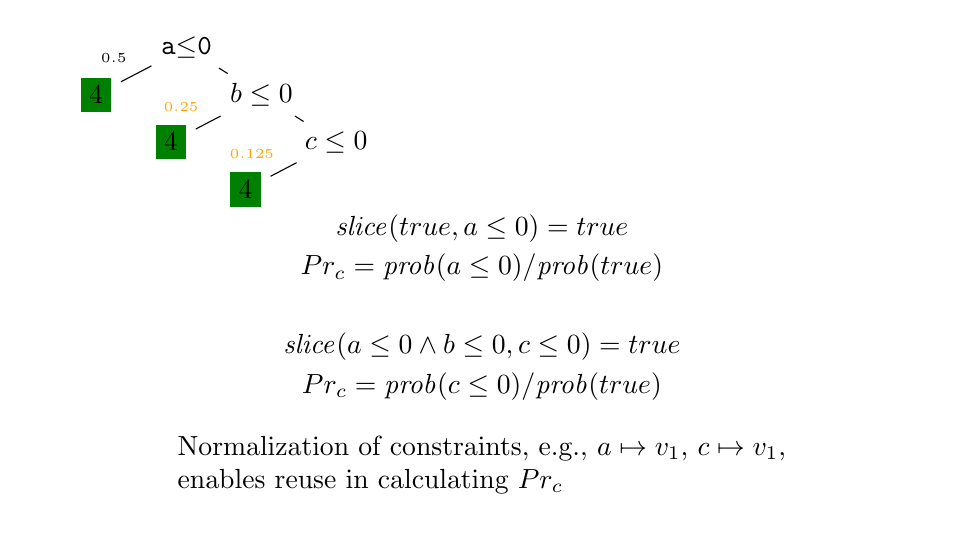
\begin{tikzpicture}[scale=0.6]
  \node {\texttt{a$\le$0}}
     child [color=black] {
       node[xshift=-7mm, yshift=3mm] {\colorbox{Green}{4}}
       edge from parent
       node[left, yshift=2mm] {\tiny $0.5$}
     }
     child [color=black] {
       node[xshift=5mm, yshift=3mm] {$b \le 0$}
       child {
         node[xshift=-7mm, yshift=3mm] {\colorbox{Green}{4}}
         edge from parent
         node[left, yshift=2mm] {\tiny \color{Orange}{$0.25$}}
       }
       child {
         node[xshift=5mm, yshift=3mm] {$c \le 0$}
         child {
           node[name=ref, xshift=-7mm, yshift=3mm] {\colorbox{Green}{4}}
           edge from parent
           node[left, yshift=2mm] {\tiny \color{Orange}{$0.125$}}
         }
         child [color=white] {
           node[xshift=5mm, yshift=3mm] {$a=b$}
           child {
             node[xshift=-30mm, yshift=2mm] {$a=c$}
             child {
               node[xshift=-4mm, yshift=3mm] {$b=c$}
               child {
                 node[xshift=0mm, yshift=2mm] {}
                 edge from parent
               }
               child [color=white] {
                 node[xshift=0mm, yshift=2mm] {}
                 edge from parent
               }
               edge from parent
             }
             child {
               node[xshift=4mm, yshift=3mm] {$b=c$}
               child [color=white] {
                 node[xshift=-2mm, yshift=2mm] {}
                 edge from parent
               }
               child { 
                 node[xshift=-2mm, yshift=2mm] {$a+b>c$}
                 child {
                   node[yshift=2mm] {}
                   edge from parent
                 }
                 child {
                   node[yshift=2mm] {}
                   edge from parent
                 }
                 edge from parent
               }
               edge from parent
             }
             edge from parent
           }
           child {
             node[xshift=10mm, yshift=2mm] {$a=c$}
             child {
               node[xshift=-13mm, yshift=3mm] {$b=c$}
               child [color=white] {
                 node[xshift=-2mm, yshift=2mm] {}
                 edge from parent
               }
               child {
                 node[xshift=-2mm, yshift=2mm] {$a+c>b$}
                 child {
                   node[yshift=2mm] {}
                   edge from parent
                 }
                 child {
                   node[yshift=2mm] {}
                   edge from parent
                 }
                 edge from parent
               }
               edge from parent
             }
             child {
               node[xshift=20mm, yshift=3mm] {$b=c$}
               child {
                 node[xshift=-12mm, yshift=2mm] {$b+c>a$}
                 child {
                   node[yshift=2mm] {}
                   edge from parent
                 }
                 child {
                   node[yshift=2mm] {}
                   edge from parent
                 }
                 edge from parent
               }
               child {
                 node[xshift=0mm, yshift=2mm] {$a+b \le c$}
                 child {
                   node[xshift=-2mm, yshift=2mm] {}
                   edge from parent
                 }
                 child {
                   node[xshift=5mm, yshift=2mm] {$b+c \le a$}
                   child {
                     node[xshift=-5mm, yshift=2mm] {}
                     edge from parent
                   }
                   child {
                     node[xshift=0mm, yshift=2mm] {$a+c \ge b$}
                     child {
                       node[yshift=2mm] {}
                       edge from parent
                     }
                     child {
                       node[yshift=2mm] {}
                       edge from parent
                     }
                     edge from parent
                   }
                   edge from parent
                 }
                 edge from parent
               }
               edge from parent
             }
             edge from parent
           }
           edge from parent
         }
         edge from parent
       }
       edge from parent
     };

   \begin{pgfonlayer}{foreground}
      \pause
      \node[name=first, yshift=5mm, xshift=30mm, below of=ref] 
         {$\x{slice}( true, a\le0) = true$};\pause
      \node[name=second, below of=first, yshift=5mm] 
         {$Pr_c = \x{prob}(a \le 0)/\x{prob}(true)$};\pause
      \node[name=third, below of=second] 
         {$\x{slice}( a\le0 \wedge b\le0, c\le0) = true$};\pause
      \node[name=fourth, below of=third, yshift=5mm] 
         {$Pr_c = \x{prob}(c \le 0)/\x{prob}(true)$};\pause
      \node[name=fourth, below of=fourth, align=left] 
         {Normalization of constraints, e.g., $a \mapsto v_1$, $c \mapsto v_1$,\\ 
enables reuse in calculating $Pr_c$};
   \end{pgfonlayer}

\end{tikzpicture}
\end{center}
\end{frame}

\begin{frame}{Calculating $\x{prob}(\cdot)$}
Linear integer arithmetic (LIA) constraints can be counted
using LattE
\begin{itemize}
\item computes the number of {\em lattice} points in 
a convex polytope;
\item constraints encoded as system of inequalities, $A x \le B$; 
\item does not support disjunction or disequality constraints, i.e., $x \not= c$
\end{itemize}
\pause
\vfill
Calculation relies on ``counting'' the number of solutions of a set
of related constraints using LattE and combining the results.
\begin{itemize}
\item $\x{count} = \x{count}_{\wedge}(\bigwedge_{\x{ineqSet}}) - \x{count}_{\vee}(\bigvee_{\x{exSet}})$
\item \texttt{return} $\x{count} / \prod_{v \in \x{vars}} \x{dom}(v)$
\end{itemize}
\end{frame}

\begin{frame}{$\alpha \wedge (x \not= 0) \wedge (y \not=0)$ cannot be expressed directly}
\begin{center}

\def\firstcircle{(0,0) circle (1.5cm)}
\def\secondcircle{(45:2cm) circle (1.5cm)}
\def\thirdcircle{(0:2cm) circle (1.5cm)}

\begin{tikzpicture}[scale=1.0]
\pause
    \draw \firstcircle node[below] {$\alpha$};
    \node[yshift=-30mm] {Count the solutions to $\alpha$};

\end{tikzpicture}
\end{center}
\end{frame}

\begin{frame}{$\alpha \wedge (x \not= 0) \wedge (y \not=0)$ cannot be expressed directly}
\begin{center}

\def\firstcircle{(0,0) circle (1.5cm)}
\def\secondcircle{(45:2cm) circle (1.5cm)}
\def\thirdcircle{(0:2cm) circle (1.5cm)}

\begin{tikzpicture}[scale=1.0]
    \draw \firstcircle node[below] {$\alpha$};
    \draw \secondcircle node [above] {$x=0$};

    \begin{scope}
      \clip \firstcircle;
      \fill[red] \secondcircle;
    \end{scope}
    \node[yshift=-30mm] {Remove the count of solutions to $\alpha \wedge (x=0)$};

\end{tikzpicture}
\end{center}
\end{frame}

\begin{frame}{$\alpha \wedge (x \not= 0) \wedge (y \not=0)$ cannot be expressed directly}
\begin{center}
\def\firstcircle{(0,0) circle (1.5cm)}
\def\secondcircle{(45:2cm) circle (1.5cm)}
\def\thirdcircle{(0:2cm) circle (1.5cm)}

\begin{tikzpicture}[scale=1.0]
    \draw \firstcircle node[below] {$\alpha$};
    \draw \thirdcircle node [below] {$y=0$};

    \begin{scope}
      \clip \firstcircle;
      \fill[blue] \thirdcircle;
    \end{scope}
    \node[yshift=-30mm] {Remove the count of solutions to $\alpha \wedge (y=0)$};

\end{tikzpicture}
\end{center}
\end{frame}


\begin{frame}{$\alpha \wedge (x \not= 0) \wedge (y \not=0)$ cannot be expressed directly}
\begin{center}
\def\firstcircle{(0,0) circle (1.5cm)}
\def\secondcircle{(45:2cm) circle (1.5cm)}
\def\thirdcircle{(0:2cm) circle (1.5cm)}

\begin{tikzpicture}[scale=1.0]
    \draw \firstcircle node[below] {$\alpha$};
    \draw \secondcircle node [above] {$x=0$};
    \draw \thirdcircle node [below] {$y=0$};

    \begin{scope}
      \clip \firstcircle;
      \clip \secondcircle;
      \fill[green] \thirdcircle;
    \end{scope}
    \node[yshift=-30mm] {Add back the count of solutions to $\alpha \wedge (x=0) \wedge (y=0)$};

\end{tikzpicture}
\end{center}
\end{frame}

\begin{frame}{$\alpha \wedge (x \not= 0) \wedge (y \not=0)$ cannot be expressed directly}
\begin{center}
\def\firstcircle{(0,0) circle (1.5cm)}
\def\secondcircle{(45:2cm) circle (1.5cm)}
\def\thirdcircle{(0:2cm) circle (1.5cm)}

\begin{tikzpicture}[scale=1.0]
    \begin{scope}
        \begin{scope}[even odd rule]% first circle without the second
            \clip \secondcircle (-3,-3) rectangle (3,3);
            \clip \thirdcircle (-3,-3) rectangle (3,3);
        \fill[yellow] \firstcircle;
        \end{scope}
        \draw \firstcircle node {$\alpha$};
        \draw \secondcircle node[yshift=5mm] {$x=0$};
        \draw \thirdcircle node[yshift=-5mm] {$y=0$};
    \end{scope}
       \node[name=ref, below, yshift=-20mm] {This results in the count of $\alpha \wedge (x\not=0) \wedge (y\not=0)$};
\pause
       \node[below of=ref, yshift=5mm] {Complexity is exponential in number of disequality constraints};
    
\end{tikzpicture}
\end{center}
\end{frame}

\begin{frame}{Optimizing $\x{count}_{\wedge}(\cdot)$}
\vfill
experience with LattE revealed that its execution time
\begin{itemize}
\item is not dependent on the size of variable domains;
\item is highly dependent on the number of variables (dimension of the polytope);
\item is highly dependent on the number of constraints (faces of the polytope);
\end{itemize}
\pause
\vfill
Experience with sliced PCs revealed that
\begin{itemize}
\item a significant portion of the PC, and many variables, can be eliminated;
\item sliced PCs, if normalized, recur throughout the symbolic execution tree
\end{itemize}
\pause
\vfill
Implementation of $\x{count}_{\wedge}(\cdot)$: Visser et al (FSE'12)
\begin{itemize}
\item normalizes the inequality system
\item caches the counts computed for each system; and 
\item checks the cache before invoking LattE.
\end{itemize}
\end{frame}

\begin{frame}{\textbf{Partial} Probabilistic symbolic execution}
\begin{center}
\pgfdeclarelayer{foreground}
\pgfsetlayers{main,foreground}
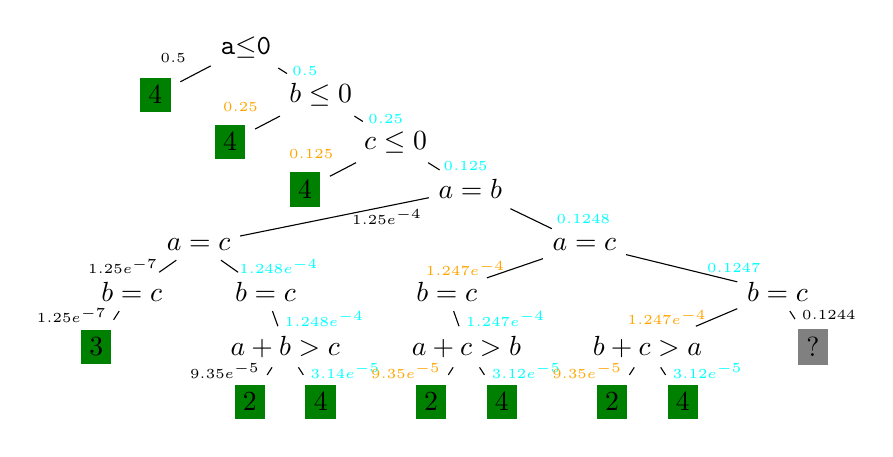
\begin{tikzpicture}[scale=0.6]
  \node {\texttt{a$\le$0}}
     child [color=black] {
       node[xshift=-7mm, yshift=3mm] {\colorbox{Green}{4}}
       edge from parent
       node[left, yshift=2mm] {\tiny $0.5$}
     }
     child [color=black] {
       node[xshift=5mm, yshift=3mm] {$b \le 0$}
       child {
         node[xshift=-7mm, yshift=3mm] {\colorbox{Green}{4}}
         edge from parent
         node[left, yshift=2mm] {\tiny \color{Orange}{$0.25$}}
       }
       child {
         node[xshift=5mm, yshift=3mm] {$c \le 0$}
         child {
           node[xshift=-7mm, yshift=3mm] {\colorbox{Green}{4}}
           edge from parent
           node[left, yshift=2mm] {\tiny \color{Orange}{$0.125$}}
         }
         child {
           node[xshift=5mm, yshift=3mm] {$a=b$}
           child {
             node[xshift=-30mm, yshift=2mm] {$a=c$}
             child {
               node[xshift=-4mm, yshift=3mm] {$b=c$}
               child {
                 node[xshift=0mm, yshift=2mm] {\colorbox{Green}{3}}
                 edge from parent
                 node[left] {\tiny $1.25e^{-7}$}
               }
               child [color=white] {
                 node[xshift=0mm, yshift=2mm] {\colorbox{white}{\textcolor{white}{3}}}
                 edge from parent
               }
               edge from parent
               node[left] {\tiny $1.25e^{-7}$}
             }
             child {
               node[xshift=4mm, yshift=3mm] {$b=c$}
               child [color=white] {
                 node[xshift=-2mm, yshift=2mm] {\colorbox{white}{\textcolor{white}{3}}}
                 edge from parent
               }
               child { 
                 node[xshift=-2mm, yshift=2mm] {$a+b>c$}
                 child {
                   node[yshift=2mm] {\colorbox{Green}{2}}
                   edge from parent
                   node[left] {\tiny $9.35e^{-5}$}
                 }
                 child {
                   node[yshift=2mm] {\colorbox{Green}{4}}
                   edge from parent
                   node[right] {\tiny \color{Cyan}{$3.14e^{-5}$}}
                 }
                 edge from parent
                 node[right] {\tiny \color{Cyan}{$1.248e^{-4}$}}
               }
               edge from parent
               node[right] {\tiny \color{Cyan}{$1.248e^{-4}$}}
             }
             edge from parent
             node[right, xshift=1mm] {\tiny {$1.25e^{-4}$}}
           }
           child {
             node[xshift=10mm, yshift=2mm] {$a=c$}
             child {
               node[xshift=-13mm, yshift=3mm] {$b=c$}
               child [color=white] {
                 node[xshift=-2mm, yshift=2mm] {\colorbox{white}{\textcolor{white}{3}}}
                 edge from parent
               }
               child {
                 node[xshift=-2mm, yshift=2mm] {$a+c>b$}
                 child {
                   node[yshift=2mm] {\colorbox{Green}{2}}
                   edge from parent
                   node[left] {\tiny \color{Orange}{$9.35e^{-5}$}}
                 }
                 child {
                   node[yshift=2mm] {\colorbox{Green}{4}}
                   edge from parent
                   node[right] {\tiny \color{Cyan}{$3.12e^{-5}$}}
                 }
                 edge from parent
                 node[right] {\tiny \color{Cyan}{$1.247e^{-4}$}}
               }
               edge from parent
               node[left] {\tiny \color{Orange}{$1.247e^{-4}$}}
             }
             child {
               node[xshift=20mm, yshift=3mm] {$b=c$}
               child {
                 node[xshift=-12mm, yshift=2mm] {$b+c>a$}
                 child {
                   node[yshift=2mm] {\colorbox{Green}{2}}
                   edge from parent
                   node[left] {\tiny \color{Orange}{$9.35e^{-5}$}}
                 }
                 child {
                   node[yshift=2mm] {\colorbox{Green}{4}}
                   edge from parent
                   node[right] {\tiny \color{Cyan}{$3.12e^{-5}$}}
                 }
                 edge from parent
               node[left] {\tiny \color{Orange}{$1.247e^{-4}$}}
               }
               child {
                 node[xshift=0mm, yshift=2mm] {\colorbox{gray}{?}}
                 edge from parent
                 node[right] {\tiny \color{black}{$0.1244$}}
               }
               edge from parent
               node[right,xshift=2mm] {\tiny \color{Cyan}{$0.1247$}}
             }
             edge from parent
             node[right,xshift=2mm] {\tiny \color{Cyan}{$0.1248$}}
           }
           edge from parent
           node[right] {\tiny \color{Cyan}{$0.125$}}
         }
         edge from parent
         node[right] {\tiny \color{Cyan}{$0.25$}}
       }
       edge from parent
       node[right] {\tiny \color{Cyan}{$0.5$}}
     };
\end{tikzpicture}
\end{center}

\end{frame}

\ignore{
\begin{frame}{Memoization and Slicing are key}
\begin{center}
\begin{itemize}
\item Ran on Binomial Heap and TreeMap collections with all possible input sequences (adds, removes, etc.) of length 4;
\item times reported in seconds\pause
\end{itemize}
\vfill
{\footnotesize
\begin{tabular}{cccccccccc}
\hline
Subject  & Memoize & Slice & PC & Var & $\x{prob}(\cdot)$ & LattE & Reused & LattE & Total \\ 
& & & Red. & Red.  & & & & time & time \\ \hline
Binomial & \ON         & \ON     & $55\%$ & $67\%$   & $634$ & $~~518$ & $~370$   & $~~35$ & $~~57$ \\         & \OF         & \ON     & $55\%$ & $67\%$   & $634$ & $~~888$ & $~~~0$ 
  & $~~61$ & $~~84$ \\
         & \ON         & \OF     & $~0\%$ & $~0\%$   & $634$ & $~3160$ & $~698$   & $~388$ & $~414$ \medskip\\TreeMap  & \ON         & \ON     & $44\%$ & $55\%$   & $766$ & $~2264$ & $~562$   & $~118$ & $~145$ \\         & \OF         & \ON     & $44\%$ & $55\%$   & $766$ & $~2826$ & $~~~0$   & $~150$ & $~178$ \\
         & \ON         & \OF     & $~0\%$ & $~0\%$   & $766$ & $12108$ & $4965$   & $1028$ & $1056$ \\
\hline
\end{tabular}
}
\end{center}
\end{frame}

\begin{frame}{Probabilistic Symbolic Execution for Concurrency}
\vfill
Non-deterministic choice is used to model a lack of information
\begin{itemize}
\item e.g., details of OS scheduling algorithm
\end{itemize}
\pause
\vfill
Two additional challenges
\begin{itemize}
\item What conditional probability should we use for a non-deterministic choice?
\item State space explosion
\end{itemize}
\vfill
We use a sampling-based analysis with reinforcement learning
\vfill
\end{frame}
}

\begin{frame}{Probabilistic Symbolic Execution for Concurrency}
\vfill
View program's behavior as a tree-structured Markov Decision Process
\begin{itemize}
\item symbolic execution tree with non-deterministic choice nodes
\end{itemize}
\pause
\vfill
Randomly sample paths, but unlike Monte Carlo methods
\begin{itemize}
\item each sampled path, $p$, contributes mass proportional to $count(PC_p)$ 
\item a sampled path is biased against being revisited
\end{itemize}
\vfill
\pause
We compute the maximum probability of an event (e.g., \texttt{assert})
\begin{itemize}
\item resolve non-deterministic choice to use max probability of child
\item calculation is bottom up like value-iteration
\end{itemize}
\vfill
\pause
MDP support works for any source of non-determinism, e.g., abstract post, unknown input values
\pause
\vfill
Fastest and most precise method to date by exploiting tree structure
\vfill
\end{frame}

\begin{frame}{Probabilistic symbolic execution algorithm} 
\vfill
The briefing paper describes a broader family of such algorithms
\vfill
\begin{minipage}{0.5\textwidth}
\begin{algorithm}[H]
\floatname{algorithm}{Alg.}
\caption{{\tt pse}$(l,m,pc)$}
\label{alg-pse}
\begin{algorithmic}
 \REPEAT
  \STATE $p \gets {\tt symsample}(l_0, m_0, \x{true})$
  \STATE $\x{processPath}(p)$
 \UNTIL {$\x{stoppingSearch}(p)$}
\end{algorithmic}
\end{algorithm}
\end{minipage}%
\begin{minipage}{0.5\textwidth}
\begin{algorithm}[H]
\floatname{algorithm}{Alg.}
\caption{{\tt symsample}$(l,m,pc)$}
\label{alg-symsample}
\begin{algorithmic}
 \IF{$\x{stoppingPath}(pc)$}
 \RETURN $pc$
 \ENDIF
 \WHILE{$\neg branch(l)$}
   \STATE $m \gets op(l)(m)$
   \STATE $l \gets succ(l)$
 \ENDWHILE

 \STATE $c \gets \x{cond}(l)(m)$

 \IF{$\x{selectBranch}(c,pc)$}
   \RETURN {\tt symsample}$(\x{succ_t}(l), m, pc \wedge c)$
 \ELSE
   \RETURN {\tt symsample}$(\x{succ_f}(l), m, pc \wedge \neg c)$
 \ENDIF
\end{algorithmic}
\end{algorithm}
\end{minipage}
\vfill
\end{frame}


\begin{frame}{Solution space quantification}
\vfill
In the 1990s ``propositional'' SAT solver technology advanced
\begin{itemize}
\item increased in performance by orders of magnitude
\item was subsequently applied to many many problems
\end{itemize}
\vfill
\pause
In the 2000s satisfiability modulo-theories (SMT) solver technology advanced
\begin{itemize}
\item increased in performance by orders of magnitude
\item was subsequently applied to many many problems
\item subsumes propositional SAT, so jump straight into SMT
\item tons of tools, e.g., Z3, Yices, CVC4, ...
\end{itemize}
\vfill
\pause
The 2010s is the decade of model counting
\vfill
Get on board early and leverage it in your research!
\vfill
\end{frame}

\begin{frame}{Exact Counting Methods}
\vfill
Believe it or not you can count the \textbf{exact} 
number of solutions of very complex systems of constraints.
\vfill
\pause
Linear constraints over integer program variables
\begin{itemize}
\item every constraint introduces a cutting plane
\item together these form a convex polyhedra
\item tools exist to exactly count the number of integer values in the interior of the polyhedra, e.g., Latte, barvinok, ...
\item scales to 10s of dimensions 
\item efficiency is \textbf{not} dependent on the size of the domain, i.e., you can solve constraints over $[MININT,MAXINT]$
\end{itemize}
\vfill
\pause
Techniques for strings, data structures, and more
\begin{itemize}
\item see the work of Luu et al (PLDI'14), Fredrickson et al (LICS'14), Freemont et al (SMT'14), Filieri et al (SPIN'15), Aydin et al (CAV'15) 
\end{itemize}
\vfill
\end{frame}

\begin{frame}{Approximate Counting Methods}
\vfill
Building on the significant literature in Monte Carlo estimation from Statistics, Physics, AI, ...
\pause
\vfill
Sampling techniques serve to estimate the parameters of a distribution
\begin{itemize}
\item rich collection of techniques for handling uniform distributions
\item number of samples needed to achieve a level of accuracy can be computed
\item a wide range of distributions can be reduced to uniform through inverse transform sampling 
\item sample uniform distribution then use hill climbing on the monotone $CDF^{-1}$
\end{itemize}
\vfill
\pause
Techniques that exploit the structure of programs are starting to appear
\begin{itemize}
\item see the work of Borges et al (PLDI'14), Borges et al (ESEC/FSE'15), ...
\end{itemize}
\vfill
\pause
Lots of room for creative blending of techniques ...
\begin{itemize}
\item model counting + search + numerical optimization : Dingel at al (FSE'14)
\end{itemize}
\vfill
\end{frame}

\end{document}
